\documentclass{scrartcl}
\usepackage{polyglossia}
\setmainlanguage[babelshorthands=true,spelling=new]{german}
\usepackage{amsmath,amssymb}
\usepackage{commath}
\usepackage{mathtools}
\usepackage{tikz}
\usepackage{pgfplots}
\pgfplotsset{compat=1.9}

\usepackage{unicode-math}
\setmainfont[
  Mapping=tex-text,
  Numbers=OldStyle
]{Libertinus Serif}
\setsansfont[
  Mapping=tex-text,
  Numbers=OldStyle
]{Libertinus Sans}
\setmathfont[AutoFakeBold]{Libertinus Math}
\setmonofont{Libertinus Mono}

%\usepackage{fontspec}
%\setmainfont{Minion Pro}
%\setsansfont{Myriad Pro}
%\usepackage[onlymath,mathlf,mathtabular,openg,minionint]{MinionPro}

\usepackage{microtype}

\KOMAoption{DIV}{calc}

\allowdisplaybreaks
\newcommand{\R}{\mathbb{R}}

\begin{document}

\title{Integral der Gauß-Funktion}
\author{Sebastian Schweikl}

%\maketitle

Die Gauß-Funktion ist definiert als
\[
  f(x) = \exp(-x^{2}), \quad x \in \mathbb{R}.
\]
Abbildung~\ref{fig:gaussian} zeigt ausschnitthaft den Verlauf der Funktion.
\begin{figure}[ht]
  \centering
  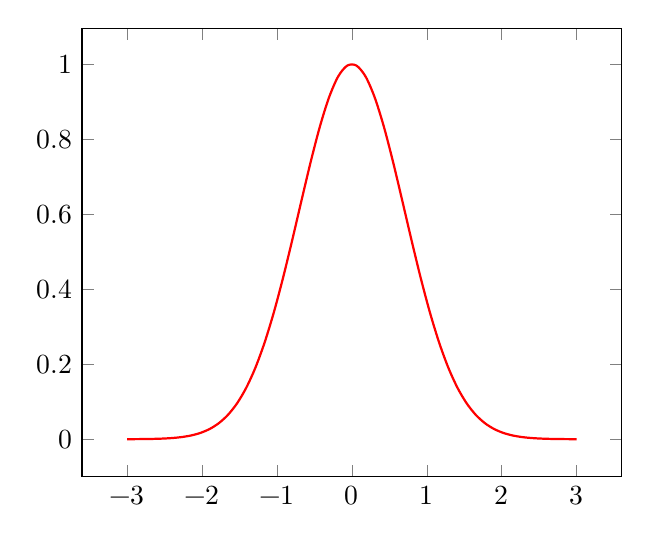
\begin{tikzpicture}
  \begin{axis}
    \addplot [domain=-3:3, mark=none, color=red, thick, samples=50, smooth] {exp(-x^2)};
  \end{axis}
  \end{tikzpicture}
  \caption{Funktionsplot der Gauß-Funktion auf dem Intervall $ [-3, 3] $. 
    Für $ x \rightarrow \pm \infty $ strebt die Funktion gegen $ 0 $.}
  \label{fig:gaussian}
\end{figure}
Es ist offensichtlich, dass $ f $ stetig auf ganz $ \R $ ist und unendlichen Träger besitzt, da die 
Funktion für alle $ x \in \R $ ungleich $ 0 $ ist. Die Frage, die sich nun stellt, ist: »Wie groß 
ist die Fläche, die zwischen der $ x $-Achse und der Gauß-Funktion eingeschlossen wird?« Um dies 
herauszufinden, müssen wir die Funktion uneigentlich integrieren. Es wird nun gezeigt, dass das 
Integral $ I $ definiert durch
\[
  I \coloneqq \int_{- \infty}^{\infty} f(x) \dif x = \int_{- \infty}^{\infty} \exp(-x^{2}) \dif x
\]
absolut konvergiert und dass $ f $ damit eine $ L_{1}(\R) $ Funktion ist. Dazu schätzen wir die 
Gauß-Funktion nach oben ab durch
\[
  g(x) \coloneqq \begin{cases}
    -x \cdot \exp(-x^{2}), & x < -1, \\
    \exp(-x^{2}),          & -1 \leq 0 \leq 1, \\
    x \cdot \exp(-x^{2}),  & x > 1,
  \end{cases}
  \qquad x \in \R.
\]
Für alle $ x \in \R $ gilt nun $ f(x) \leq g(x) $. Abbildung~\ref{fig:approximation} 
veranschaulicht dies beispielhaft für die $ x $ aus dem Intervall $ [-3,3] $.
\begin{figure}[ht]
  \centering
  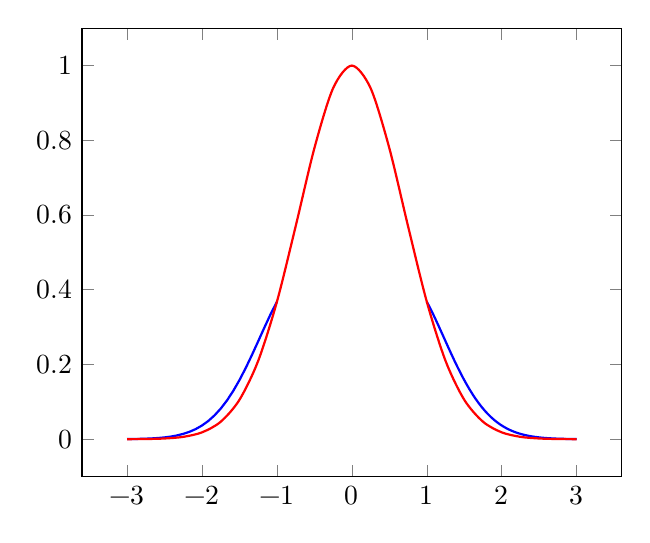
\begin{tikzpicture}
  \begin{axis}
    \addplot [domain=-3:-1, mark=none, color=blue, thick, samples=25] {-x*exp(-x^2)};
    \addplot [domain=1:3, mark=none, color=blue, thick, samples=50] {x*exp(-x^2)};
    \addplot [domain=-3:3, mark=none, color=red, thick, samples=25,smooth] {exp(-x^2)};
  \end{axis}
  \end{tikzpicture}
  \caption{Abschätzung von $ f $ (rot gezeichnet) nach oben durch $ g $ (blau gezeichnet).}
  \label{fig:approximation}
\end{figure}
Unter Verwendung der Tatsache, dass $ f(x) > 0 $ für alle $ x \in \R $, und mit der Stetigkeit und 
Symmetrie von $ g $ erhalten wir folglich
\begin{align*}
   \norm{f}_{1} 
&= \int_{-\infty}^{\infty} |\exp(-x^{2})| \dif x
 = \int_{-\infty}^{\infty} \exp(-x^{2}) \dif x \\
&\leq \int_{-\infty}^{\infty} g(x) \dif x \\
&= \int_{-\infty}^{-1} -x \exp(-x^{2}) \dif x 
   + \int_{-1}^{1} \exp(-x^{2}) \dif x
   + \int_{1}^{\infty} x \exp(-x^{2}) \dif x \\
&= \int_{-1}^{1} \exp(-x^{2}) \dif x + 2 \int_{1}^{\infty} x \exp(-x^{2}) \dif x.
\end{align*}
Wir betrachten das uneigentliche Integral $ \int_{1}^{\infty} x \exp(-x^{2}) \dif x $.
Dieses konvergiert, da der Grenzwert
\begin{align*}
   \lim\limits_{n \to \infty} \int_{1}^{n} x \exp(-x^{2}) \dif x
&= \lim\limits_{n \to \infty} \frac{1}{2} \int_{1}^{n^{2}} \exp(-u) \dif u
 = \frac{1}{2} \lim\limits_{n \to \infty} \eval[3]{-\exp(-u)}_{1}^{n^{2}} \\
&= \frac{1}{2} \lim\limits_{n \to \infty} - \exp(-n^{2}) - (-\exp(-1)) \\
&= \left( \frac{1}{2} + \exp(-1) \right) 
      \lim\limits_{n \to \infty} \underbrace{-\exp(-n^{2})}_{\to 0}
 = \frac{1}{2} + \exp(-1)
\end{align*}
existiert. Man beachte dabei die Substitution $ u \coloneqq x^{2} $, $ \dif u = 2x \dif x $. Daraus
folgt nun
\[
  \norm{f}_{1} < \infty.
\]
Also ist $ f $ integrierbar und daher dürfen wir den Wert von $ I $ darstellen durch die Berechnung
\[
  I = \lim\limits_{n \to \infty} I_{n} \coloneqq 
  \lim\limits_{n \to \infty} \int_{-n}^{n} f(x) \dif x.
\]
Da in jedem Fall $ I_{n} \geq 0 $ gilt, ist Quadrieren eine Äquivalenzumformung und man darf 
schreiben
\[
  I_{n} = \sqrt{ (I_{n})^{2} }.
\]
Da zudem $ f $ auf dem Kompaktum $ [-n, n] $ integriert wird, kann der Satz von Fubini angewendet
werden, um die Integrationsreihenfolge zu vertauschen. Dies rechtfertigt
\[
  (I_{n})^{2}
= \left( \int_{-n}^{n} f(x) \dif x \right) \left( \int_{-n}^{n} f(y) \dif y \right)
= \int_{-n}^{n} \int_{-n}^{n} \exp(-(x^{2} + y^{2})) \dif x \dif y.
\]
Wie man sieht, wurde von einem eindimensionalen Integral auf ein zweidimensionales Integral 
übergegangen. Abbildung~\ref{fig:gaussian3d} zeigt den Integranden, welcher nun die Gauß-Funktion
in zwei Variablen ist.
\begin{figure}[ht]
\centering
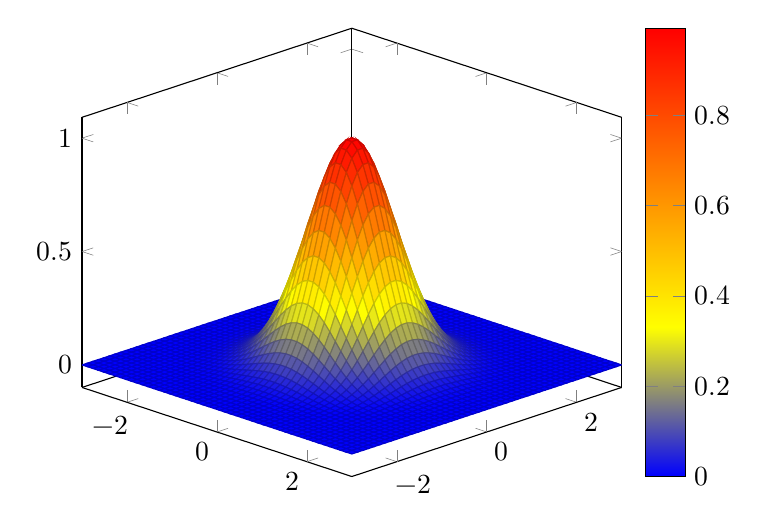
\begin{tikzpicture}
  \begin{axis}[grid style={dashed, gray!30}, colorbar, view={45}{25}]
  \addplot3 [surf, domain=-3:3, domain y=-3:3, samples=50] {exp(-( x^2 + y^2) )};
  \end{axis}
\end{tikzpicture}
\caption{3D-Plot der Gauß-Funktion in zwei Variablen auf dem Intervall $ [-3,3] \times [-3,3] $.}
\label{fig:gaussian3d}
\end{figure}
Die Integration in zwei Variablen und die Rotationssymmetrie des Integranden legen einen 
Wechsel zu Polarkoordinaten nahe, indem wir den Transformationssatz für Integrale in mehreren 
Variablen anwenden. Wir definieren eine Funktion
\[
  \Phi \colon [0, \infty) \times [0, 2\pi) \rightarrow \R \times \R, \quad
  (r, \vartheta) \mapsto (x \coloneqq r \cos(\vartheta), y \coloneqq r \sin(\vartheta)),
\]
welche die gegebenen Polarkoordinaten mit Radius $ r $ und Winkel $ \vartheta $ in kartesische 
Koordinaten $ (x, y) $ umwandelt. Das bedeutet, anstatt über Quadrate wollen wir nun über Kreise 
integrieren. Das Volumen der Funktion über einem Quadrat kann nach oben durch das Volumen über dem 
Umkreis und nach unten durch das Volumen über Inkreis dieses Quadrats beschränkt werden. Siehe 
hierfür auch Abbildung~\ref{fig:square}.
\begin{figure}[ht]
\begin{captionbeside}{Die Fläche des roten Quadrats mit Seitenlänge $ 2n $ lässt sich nach oben 
durch die Fläche des Umkreises mit Radius $ 2\sqrt{n} $ und nach unten durch die Fläche des 
Inkreises mit Radius $ n $ beschränken.}[l]
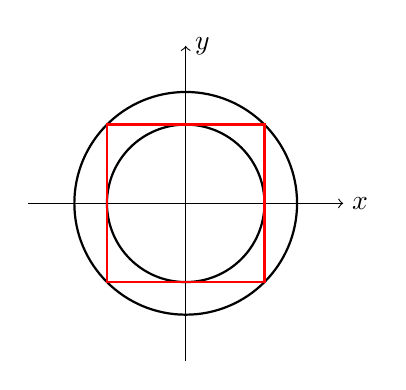
\begin{tikzpicture}
%\draw [color=gray, very thin] (-3.5,-3.5) grid (3.5,3.5);
\draw [->] (-2,0) -- (2,0) node [right] {$ x $};
\draw [->] (0,-2) -- (0,2) node [right] {$ y $};
\draw [thick] (0,0) circle (1);
\draw [thick] (0,0) circle ({sqrt(2)});
\draw [color=red,thick] (-1,-1) rectangle (1,1);
\end{tikzpicture}
\end{captionbeside}
\label{fig:square}
\end{figure}
Wir berechnen zunächst das Volumen über dem Inkreis. Die Jacobi-Matrix von $ \Phi $ ist gegeben 
durch
\[
  J_{\Phi} = \begin{pmatrix}
    \dpd{\Phi_{1}}{r}(r, \vartheta) & \dpd{\Phi_{1}}{\vartheta}(r, \vartheta) \\[1em]
    \dpd{\Phi_{2}}{r}(r, \vartheta) & \dpd{\Phi_{2}}{\vartheta}(r, \vartheta)
  \end{pmatrix}
  = \begin{pmatrix}
    \cos(\vartheta) & -r \sin(\vartheta) \\
    \sin(\vartheta) &  r \cos(\vartheta)
  \end{pmatrix}
\]
mit der Funktionaldeterminante
\[
    \det(J_{\Phi})
  = r \cos^{2}(\vartheta) + r \sin^{2}(\vartheta)
  = r (\cos^{2}(\vartheta) + \sin^{2}(\vartheta))
  = r.
\]
Aus der Formel für $ (I_{n})^{2} $ erhält man mittels Variablensubstitution von
$ x = r \cos(\vartheta) $ und
$ y = r \sin(\vartheta) $ das Integral
\begin{align*}
V_{I}(n) \coloneqq{}& \int_{0}^{2\pi} \int_{0}^{n} |r|
      \exp\left(- \left( r^{2} \cos^{2}(\vartheta) + r^{2} \sin^{2}(\vartheta) \right) \right) 
      \dif r \dif \vartheta \\
={}& \int_{0}^{2\pi} \int_{0}^{n} r \exp(- r^{2} ) \dif r \dif \vartheta \\
={}& \left( \int_{0}^{2\pi} \dif \vartheta \right) 
            \left( \int_{0}^{n} r \exp(- r^{2} ) \dif r \right) \\
={}& 2\pi \int_{0}^{n} r \exp(- r^{2} ) \dif r .
\end{align*}
Um das verbleibende Integral auszuwerten, setze $ u = r^{2} $. Dann ist $ \dif u = 2r \dif r $. 
Substitution liefert weiter
\begin{align*}
   2\pi \int_{0}^{n} r \exp(- r^{2} ) \dif r
&= \pi \int_{0}^{n^{2}} \exp(- u ) \dif u
 = \pi \eval[3]{\left( -\exp(-u) \right)}_{u = 0}^{n^{2}} \\
&= \pi (-\exp(-n^{2}) + 1).
\end{align*}
Analog erhält man für das Volumen über dem Umkreis
\[
  V_{U}(n) \coloneqq \pi (-\exp(-2n^{2}) + 1).
\]
Also folglich
\[
  V_{I}(n) \leq (I_{n})^{2} \leq V_{U}(n).
\]
Lässt man $ n $ gegen unendlich gehen, so erhält man
\[
  \lim\limits_{n \to \infty} V_{I}(n)
 = \lim\limits_{n \to \infty} \pi (-\exp(-n^{2}) + 1)
 = \pi \left( \lim\limits_{n \to \infty} -\exp(-n^{2}) + 1 \right)
 = \pi
\]
und wiederum analog für das Volumen über dem Umkreis
\[
  \lim\limits_{n \to \infty} V_{U}(n) = \pi.
\]
Mit dem Einschnürungssatz folgt dann, dass auch
\[
  \lim\limits_{n \to \infty} (I_{n})^{2} = \pi
\]
gelten muss. Es folgt schließlich
\[
  I = \int_{\R} \exp(-x^{2}) \dif x = \sqrt{ \lim\limits_{n \to \infty} (I_{n})^{2} } = \sqrt{\pi}.
\]

Alternativer, kurzer Beweis: Aus der Stochastik ist die Wahrscheinlichkeitsdichte der 
Standardnormalverteilung
\[
  \phi(x) = \frac{1}{\sqrt{2 \pi}} \exp \left( - \frac{x^{2}}{2} \right)
\]
mit der Eigenschaft
\[
  \int_{\R} \phi(x) \dif x = 1
\]
bereits bekannt. Substitution von $ u = x / \sqrt{2} $, $ \dif x = \sqrt{2} \dif u $ führt zu
\[
    \int_{\R} \frac{1}{\sqrt{2 \pi}} \exp \left( - \frac{x^{2}}{2} \right) \dif x
  = \int_{\R} \frac{1}{\sqrt{\pi}} \exp(-u^{2}) \dif u
  = 1 \quad \Leftrightarrow \quad
    \int_{\R} \exp(-u^{2}) \dif u = \sqrt{\pi}.
\]
\end{document}